\documentclass{article}

\usepackage{amsmath,bm}
\usepackage{tikz}

\begin{document}

\begin{equation}
{\color{blue}\bm{\xi}} = -\bm{\mu} + {\color{red}\bm{\eta}}
\end{equation}


\subsection{tria}

\newcommand{\commontri}{
\path [draw=gray] (1,0) -- (1,1) -- (0,1) -- (-1,0) -- (-1,-1) -- (0,-1) -- cycle;
\path [draw=gray] (-1,0) -- (1,0);
\path [draw=gray] (0,-1) -- (0,1);
\path [draw=gray] (-1,-1) -- (1,1);
\path [draw, ->] (-.2,0) -- (1.2,0) node [anchor = west] {$\xi_1$};
\path [draw, ->] (0,-.2) -- (0,1.2) node [anchor = south] {$\xi_2$};
\path [fill=red, opacity=.5] (0-\m,0-\p) -- (1-\m,0-\p) -- (1-\m,1-\p) -- cycle;
\path [fill = blue, opacity=.5] (0,0) -- (1,0) -- (1,1) -- cycle;
\path [draw, fill] (\m,\p) circle(.03) -- (-\m,-\p) circle(.03);
}


\subsubsection{Domain I.}
%
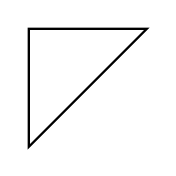
\begin{tikzpicture}[scale=1.5]
\def\m{-.5}
\def\p{-.3}
\commontri
\path [draw, thick] (0,0) -- (-1,0) -- (-1,-1) -- cycle;
\end{tikzpicture}
%
\begin{align}
-\mu_1 &< \xi_1 < 1 \nonumber \\
-\mu_2 &< \xi_2 < -\mu_2 + \xi_1+\mu_1 \nonumber
\end{align}


\subsubsection{Domain II.}
%
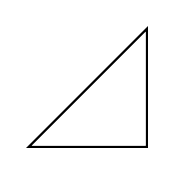
\begin{tikzpicture}[scale=1.5]
\def\m{.6}
\def\p{.3}
\commontri
\path [draw, thick] (0,0) -- (1,0) -- (1,1) -- cycle;
\end{tikzpicture}
%
\begin{align}
0 &< \xi_1 < 1-\mu_1 \nonumber \\
0 &< \xi_2 < \xi_1 \nonumber
\end{align}



\subsubsection{Domain III.}
%
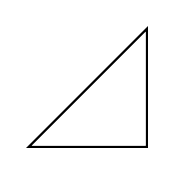
\begin{tikzpicture}[scale=1.5]
\def\m{-.3}
\def\p{.5}
\commontri
\path [draw, thick] (0,0) -- (0,1) -- (-1,0) -- cycle;
\end{tikzpicture}
%
\begin{align}
\mu_2-\mu_1 &< \xi_1 < 1 \nonumber \\
0 &< \xi_2 < \xi_1 - \mu_2+\mu_1\nonumber
\end{align}




\subsubsection{Domain IV.}
%
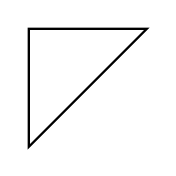
\begin{tikzpicture}[scale=1.5]
\def\m{.3}
\def\p{-.5}
\commontri
\path [draw, thick] (0,0) -- (0,-1) -- (1,0) -- cycle;
\end{tikzpicture}
%
\begin{align}
-\mu_2 &< \xi_1 < 1-\mu_1 \nonumber \\
-\mu_2 &< \xi_2 < \xi_1 \nonumber
\end{align}



\subsubsection{Domain V.}
%
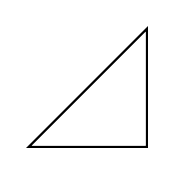
\begin{tikzpicture}[scale=1.5]
\def\m{-.3}
\def\p{-.6}
\commontri
\path [draw, thick] (0,0) -- (-1,-1) -- (0,-1) -- cycle;
\end{tikzpicture}
%
\begin{align}
-\mu_2 &< \xi_1 < 1 \nonumber \\
-\mu_2 &< \xi_2 < \xi_1 \nonumber
\end{align}


\subsubsection{Domain VI.}
%
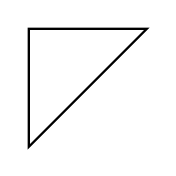
\begin{tikzpicture}[scale=1.5]
\def\m{.3}
\def\p{.6}
\commontri
\path [draw, thick] (0,0) -- (1,1) -- (0,1) -- cycle;
\end{tikzpicture}
%
\begin{align}
\mu_2-\mu_1 &< \xi_1 < 1-\mu_1 \nonumber \\
0 &< \xi_2 < \xi_1 - \mu_2+\mu_1\nonumber
\end{align}



\subsection{quad}

\newcommand{\commonquad}{
\path [draw=gray] (1,-1) -- (1,1) -- (-1,1) -- (-1,-1) -- cycle;
\path [draw=gray] (-1,0) -- (1,0);
\path [draw=gray] (0,-1) -- (0,1);
\path [draw, ->] (-1.2,0) -- (1.2,0) node [anchor = west] {$\xi_1$};
\path [draw, ->] (0,-1.2) -- (0,1.2) node [anchor = south] {$\xi_2$};
\path [fill=red, opacity=.5] (0-\m,0-\p) -- (1-\m,0-\p) -- (1-\m,1-\p) -- (0-\m,1-\p) -- cycle;
\path [fill = blue, opacity=.5] (0,0) -- (1,0) -- (1,1) -- (0,1) -- cycle;
\path [draw, fill] (\m,\p) circle(.03) -- (-\m,-\p) circle(.03);
}



\subsubsection{Domain I.}
%
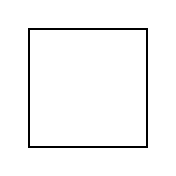
\begin{tikzpicture}[scale=1.5]
\def\m{-.3}
\def\p{-.6}
\commonquad
\path [draw, thick] (0,0) -- (-1,0) -- (-1,-1) -- (0,-1) -- cycle;
\end{tikzpicture}
%
\begin{align}
-\mu_1 &< \xi_1 < 1 \nonumber \\
-\mu_2 &< \xi_2 < 1 \nonumber
\end{align}



\subsubsection{Domain II.}
%
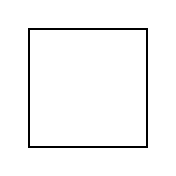
\begin{tikzpicture}[scale=1.5]
\def\m{.3}
\def\p{.6}
\commonquad
\path [draw, thick] (0,0) -- (1,0) -- (1,1) -- (0,1) -- cycle;
\end{tikzpicture}
%
\begin{align}
0 &< \xi_1 < 1 - \mu_1 \nonumber \\
0 &< \xi_2 < 1 - \mu_2 \nonumber
\end{align}


\subsubsection{Domain III.}
%
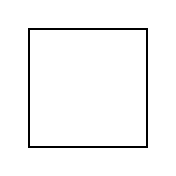
\begin{tikzpicture}[scale=1.5]
\def\m{-.3}
\def\p{.6}
\commonquad
\path [draw, thick] (0,0) -- (-1,0) -- (-1,1) -- (0,1) -- cycle;
\end{tikzpicture}
%
\begin{align}
-\mu_1 &< \xi_1 < 1 \nonumber \\
0 &< \xi_2 < 1- \mu_2 \nonumber
\end{align}


\subsubsection{Domain IV.}
%
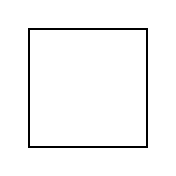
\begin{tikzpicture}[scale=1.5]
\def\m{.3}
\def\p{-.6}
\commonquad
\path [draw, thick] (0,0) -- (1,0) -- (1,-1) -- (0,-1) -- cycle;
\end{tikzpicture}
%
\begin{align}
0 &< \xi_1 < 1-\mu_1 \nonumber \\
-\mu_2 &< \xi_2 < 1 \nonumber
\end{align}





\end{document}

